
Como discutido na introdução, o nexo entre cidadãos e governo é a base dos
sistemas democráticos. Dada a importância desse nexo, não é surpresa que na
Ciência Política exista uma grande gama de trabalhos e abordagens que busquem
descrever, explicar e prever as várias dimensões desse nexo. A caracterização e
justificativa para nosso problema de pesquisa parte de um diálogo com a Teoria
Política Formal, a ser definida e discutida em seguida.

\subsection{Fundamentos da Teoria Política Formal}

Vamos definir Teoria Política Formal como: conjunto de modelos e hipóteses
teóricas explicitamente definidos que buscam representar atividades e
comportamentos relacionados à ação e escolha coletiva.

Com essa definição estamos conjugando três definições: a de Teoria, a de
Política e a de Formal. O conceito de política, e em certa medida o de teoria,
pode ser considerado como ``essencialmente contestado'', isto é, é um conceito
cuja grande importância normativa faz com que haja uma disputa em relação à sua
definição e uso\cite{collier2006essentially}. Existe assim ampla literatura
lidando com a melhor definição do que é política. Vamos usar a definição
dada por Joe Oppenheimer, para o qual  a ``política consiste
no comportamento realizado com o objetivo de tomar decisões centralizadas para
um grupo, ou para assegurar o interesse de membros desse grupo'' \cite[p.
I]{oppenheimer2012principles}\footnote{Essa definição é equivalente a dada por
  \citeonline{barber2003strong}. Para uma discussão mais aprofundada sobre o
  tema ver: \citeonline{warren1999political}.}.

Quanto a definição de teorias estamos seguindo perspectivas pós-positivistas de
ciência, particularmente a Visão Semântico-Pragmática de
\citeonline{clarke2012model} em que teorias são conjuntos de modelos, pensados
como representações de sistemas concretos, e hipóteses teóricas - a delimitação
da similaridade dos modelos com determinados sistemas alvo\footnote{Para uma
  discussão sobre as diferentes visões sobre o que são teorias e modelos ver
  \citeonline{sep-structure-scientific-theories}.}.

Por fim, entendemos que os modelos são formais na medida em que construídos por
meio de algum sistema formal \cite{wong2015formal}. Em Teoria Política Formal
isso significa que tendem a ser construídos usando o intermédio da lógica formal,
matemática ou computação \cite{morton1999methods}. Nosso foco na literatura em
teoria política formal é justificado pelo fato dela ser um corpo teórico
construído por meio de modelos \textit{explícitos} \cite{epstein2008model}, de
forma que a seguinte relação fique clara:

\begin{figure}[H]
  \centering 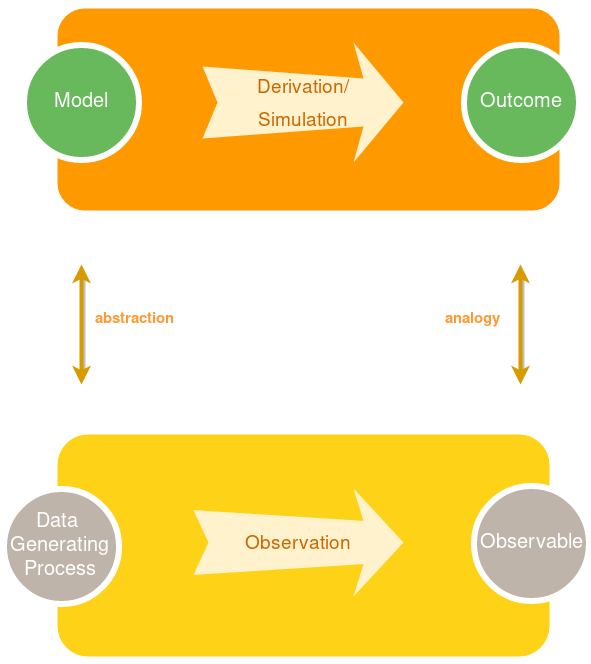
\includegraphics[scale = 0.5]{ims/ms.png}
  \caption{Relação entre Modelos e Sistemas Alvo.}
  Fonte: Adaptado de \citeonline{downey2012think}
\end{figure}


\textcolor{red}{Ficou faltando a história aqui.
  \begin{itemize}
  \item usar Mclean
  \item usar SE sobre free riding
  \item usar Ordeshook
  \end{itemize}
}


Embora não seja a única forma de se modelar formalmente fenômenos políticos,
modelos de escolha racional são em larga medida os mais comuns
\cite{austen1998social}.

De uma forma geral, os modelos da Teoria da Escolha Racional, em política,
buscam representar fenômenos segundo alguma variante da seguinte equação, a
Equação de Plott \cite{munger2015choosing, ostrom1986agenda}\footnote{Essa
  ``equação'' é conceitual. \(\oplus\) é usado como um operador abstrato não
  especificado \cite{ostrom1986agenda}. }:

\begin{align*}
  \text{Preferences} \oplus \text{Beliefs}  \oplus  \text{Physical Possibilities} \oplus \text{Institutions} = \text{Outcomes}
\end{align*}

O conjunto de modelos conhecidos como ``Teoria da Escolha Racional'' podem ser
dividido em duas variantes: \textit{thin} ou \textit{thick}
\cite{hechter1997sociological, green1996pathologies}. Ambos os tipos de modelos
são construídos com base nos pressupostos mínimos de um modelo de ator racional:
preferências racionais e racionalidade bayesiana \cite{gintis2016individuality}.
A diferença entre eles é que os modelos \textit{thin} não fazem pressupostos
substantivos sobre os valores e objetivos dos agentes. Neles os teóricos buscam
modelar a combinação entre agentes e instituições da maneira mais geral
possível. Já modelos \textit{thick} adicionam um conjunto de pressupostos extras
para representar fenômenos como o comparecimento às urnas, a competição
partidária, a escolha de candidatos pelo eleitorado, independência burocrática,
o efeito fiscal de constituições, dentre outros \cite{bendor2011behavioral}.









